%!TEX root = Manuscript.tex


\chapter{Scheduling Unsynchronized Periodic Datagrams with a single Buffer }
\label{chap:PALL}
\minitoc

This chapter is taken from a published paper~\cite{DBLP:conf/ict/BarthGLMS18} and its extended version~\cite{DBLP:journals/corr/abs-1801-07029} (except the last section).
      
         \section{Solving \texttt{PALL} on Star Routed Networks}\label{sec:PALL}
    
    In this section, we consider the more general \pall problem on star routed networks. The datagrams are allowed to wait in the BBUs to yield more possible assignments. Hence, we allow the process time of a route to be greater than the length of the route, but it must be bounded by its deadline.


	\subsection{Simple Star Routed Networks}
		

	Often in real networks, the length of the routes are not arbitrary and we may exploit that to solve \pall easily. For instance all the weights on the arcs $(c_1,c_2)$ are the same if all the BBUs are in the same data-center and all datagrams require the same time to be processed in the BBUs.
Finding an assignment in that case is trivial: send all datagrams so that they follow each other without gaps in $c_1$. In the corresponding canonical routed network, one can set $o_i = i\tau$.  Since all arcs $(c_1,c_2)$ are of weight zero in this case, the interval of time used in $c_2$ are the same as for $c_1$ and there is no collision in $c_2$.

	Another possible assumption would be that all deadlines are larger than the longest route. It may happens when, in the network we model, all RRHs are at almost the same distance to the shared link.

	 \begin{proposition}\label{prop:asym}
	Let $N = ({\cal R}, \omega)$ be a canonical star routed network with $n$ routes, let $P \geq n\tau$ and let $d$ be a deadline function. Let $r_{n-1}$ be the longest route, and assume that for all $r\in {\cal R}$, $d(r) \geq \lambda(r_{n-1})$. Then, there is a $(P,\tau)$-periodic assignment for $N$ and $d$ and it can be built in time $O(n)$.
	 \end{proposition}
      \begin{proof}
       The idea is to set the waiting times of all routes so their datagrams behave exactly as the datagram of $r_{n-1}$. The offset of the route $r_i$ is set to $i\tau$, which ensures that there is no collision in $c_1$ as soon as $P \geq n\tau$. The waiting time of the route $r_i$ is $w_i = \lambda(r_{n-1}) - \lambda(r_{i})$.
        
    The time at which the datagrams of $r_i$ arrives in $c_2$ is $t(r_i, c_2) = w_i + i\tau + \lambda(r_{i})$. Substituting $w_i$ by its value, we obtain $t(r_i, c_2) =  i\tau + \lambda(r_{n-1})$.
    Hence, there is no collision in $c_2$. We denote by $A$ the defined assignment. By definition of the transmission time, we have $TR(r_i,A) = w_i + \lambda(r_i) = \lambda(r_{n-1})$. By hypothesis, $d(r_i) \geq \lambda(r_{n-1})$, which proves that the assignment respect the deadlines.

	Finally, the complexity is in $O(n)$ since we have to find the maximum of the length of the $n$ routes and the computation of each $w_i$ is done by a constant number of arithmetic operations.
     \end{proof}
     
    
     \subsection{Two Stages Approach}
     
      We may decompose an algorithm solving \pall on a star routed network in two parts: first set all the offsets of routes so that there is no collision in $c_1$ and then knowing this information find waiting times so that there is no collision in $c_2$ while respecting the deadlines. 
      
     First, we give several heuristics to choose the offsets, which are experimentally evaluated in Section~\ref{sec:resultsPALL}. We assume that the sar routed network is in canonical form. 
      We send the datagrams through $c_1$ in a compact way (no gap between datagrams). It means that for $n$ routes, denoted by $r_0, \dots, r_{n-1}$, the offsets are $o_i = \sigma(i) \times \tau$, for some permutation $\sigma \in \Sigma_n$. We consider the following orders $\sigma$: 
	
	\begin{itemize}
	 \item Decreasing Margin (DM): Decreasing order on the margin of the routes.
	 \item Increasing Margin (IM): Increasing order on the margin of the routes. 
	 \item Decreasing Arc (DA): Decreasing order on the length of the arcs $(c_1,c_2)$.
	 \item Increasing Arc (IA): Increasing order on the length of the arcs $(c_1,c_2)$. This sending order yields a $(P,\tau)$ periodic assignment in which the waiting times are zero, if the period is large enough (see Proposition \ref{prop:SL}).
	\end{itemize}

    We also propose to fix the offsets of the routes according to some random order.
    If we pack the datagrams as previously, we call Random Order (RO) the heurisitic of chosing an order
    uniformly at random. We may also allow some time between two consecutive datagrams in $c_2$. The order of the routes in $c_1$ is still random and we consider two variations. Either the time between two datagrams in $c_1$ is random and we call this heuristic Random Order and Random Spacing (RORS) or the time between two consecutive datagrams is always the same and we call this heuristic Random Order and Balanced Spacing (ROBS).
 	
 	We call \textbf{W}aiting \textbf{T}ime \textbf{A}ssignment or \wta the problem \pall on a star routed network, whith the offsets of the routes also given as input. A solution to \wta is a valid assignment such that the offsets coincide with those given in the instance. 

   In the rest of the section we study different methods to solve \wta either by polynomial time heuristics or by an FPT algorithm. The methods to solve \wta are then combined with the heuristics proposed to fix the offsets of the routes to obtain an algorithm solving \pall.  
   
   \subsection{Greedy Scheduling of Waiting Times}

   We now solve the problem \wta, hence we are given a routed network, a deadline function and an offset for each route. The \textbf{release time} of a route is defined as the first time its datagram can go through $c_2$: for a route $r$ with offest $o_r$, it is $\lambda(r,c_2) + o_r$.

    The first algorithm we propose to solve \wta is a greedy algorithm which sets the waiting times in a greedy way, by prioritizing the routes with the earliest deadline to best satisfy the constraints on the process time. We call it \greedydeadline, and it works as follows. Set $t=0$ and $U = \cal{R}$. While there is a route in $U$, find $s \geq t$ the smallest time for which there is $r \in U$ with a release time lower or equal to $s$. If there are several routes in $U$ with a release time lower or equal  to $s$, then $r$ with the smallest deadline is selected and set $w_r = s - \lambda(r,c_2)$, $t = s + \tau$ and $ U = U \setminus \{r\}$.

    This algorithm does not take into account the periodicity, which may create collisions. Let $r_0$ be the first route selected by the algorithm, then $t_0 = t(r_0,c_2)$ is the first time at which a datagram go through $c_2$.
	Then, if all routes $r$ are such that $t(r, c_2) \leq t_0 + P - \tau$, 
	then by construction, there are no collisions on the central arc.
      However, if a route $r$ has a larger $t(r, c_2)$, since we consider everything modulo $P$ to determine collision, it may collide with another route. Therefore we correct \greedydeadline by this simple modification: $s \geq t$ is the smallest time for which there is $r \in U$ with a release time lower or equal to $s$ \emph{such that there is no collision if a datagram goes through $c_2$ at time $s$}. This rule guarantees that if \greedydeadline succeeds to set all waiting times, it finds a solution to \wta, as illustrated in Figure~\ref{fig:greedydeadline}. However, it can fails to find the value $s$ at some point because the constraint on collisions cannot be satisfied. In that case \greedydeadline stops without finding a solution.
    
    \begin{figure}
          \begin{center}
   \begin{tabularx}{0.7\textwidth}{|c|X|X|X|X|X|X|}
    \hline
     Route& $0$ & $1$ & $2$& $3$ & $4$\\
    \hline
    Deadline & $10$ &$15$&$5$&$7$&$30$\\
    \hline
     Release time & $0$ &$2$&$3$&$16$&$17$\\
    \hline
    Waiting time & $0$ &$5$&$1$&$0$&$15$\\
    \hline
      \end{tabularx}
      
      
      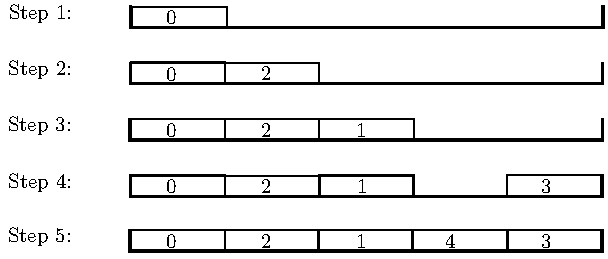
\includegraphics[width=0.7\textwidth]{Chapitre4/examplegreedy.pdf}
      \caption{A run of \greedydeadline with $P = 20, \tau = 4$.}
           \label{fig:greedydeadline}
      \end{center}
      
    \end{figure}

    %Algorithm~\ref{alg:GD} is the formal description of the previous algorithm. 
    % The function  min\_non\_assigned(eligible\_time) returns the non assigned route with the smallest time eligible time. The function update(t,free\_intervals) removes an interval of size $\tau$ beginning at t, which correspond to the datagram,  from free\_intervals.
     
    %  \begin{algorithm}\label{alg:GD}
    % \caption{ Greedy deadline ({\bf GD}) }
    % \begin{algorithmic}
    % \REQUIRE A routed network $(G,{\cal R})$, a period $P$, packet size $\tau$, the deadlines $d_i$, the offsets $m_i$
    % \ENSURE $(P,\tau)$-periodic assignment of $(G,{\cal R})$, or failure
    %\STATE  ${\cal H} \leftarrow$ empty set //{\em set of eligible routes with their deadline}
     %   \STATE  free\_ intervals $\leftarrow$ [0,$P$] //{\em list of intervals of free slots}
   
    % \FORALL{route $r_{i}$}
%      \STATE  deadline[$r_i$]  $\leftarrow$  $m_{i} + T_{max} - \Omega(s_i,c_s)$
     %\STATE  eligible\_time[$r_i$] $\leftarrow$ $m_{i} +  \lambda(r_i) + \Omega(c_t,t_i)$
     %  \ENDFOR
       
     %  \WHILE{There is some non-assigned routes}
      % \IF{${\cal H}$ is empty}
     %  \STATE $r_i$ $\leftarrow $ min\_non\_assigned(eligible\_time)
     %  \STATE insert(${\cal H}$,$r_i$,$d_i$).
     %  \ENDIF
      
      % \STATE $r \leftarrow $ extract\_min(${\cal H}$)
      % \STATE t $\leftarrow$ next\_free\_interval(free\_intervals, t) //{\em if there is no more free interval of size $\tau$, the algorithm fails}
      % \STATE $w_i \leftarrow$ t - eligible\_time[$r_i$]
      % \STATE update(t,free\_ intervals)
      % \STATE t $\leftarrow$ t + $\tau$
      % \FORALL{routes $r_i$ with  eligible\_time[$r_i$] $\leq$ t}
 	 %	\STATE insert(${\cal H}$,$r_i$).
      % \ENDFOR
      % \ENDWHILE
     %\end{algorithmic}
     %\end{algorithm}

   


    The complexity of \greedydeadline is in $O(n\log(n))$, using the proper data structures. The set of routes $\cal{R}$ must be maintained in a binary heap to be able to find the one with smallest deadline in time $O(\log(n))$. To deal with the possible collisions, one maintains a list of the intervals
    of time during which a datagram can go through $c_2$. Each time the waiting time of a route is fixed, an interval is split into at most two intervals in constant time. During the whole algorithm, each element of this list is used at most twice either when doing an insertion or when looking for the next free interval. Hence, the time needed to maintain the list is in $O(n)$. 
  
     \subsection{Earliest Deadline Scheduling}\label{sec:wtaheuristic}
     
     
     The problem \wta is the same as a classical earliest deadline scheduling problem, if we forget the periodicity. Given a set of jobs with \emph{release times} and \emph{deadlines}, schedule all jobs on a single processor, that is choose the time at which they are computed, so that no two jobs are scheduled at the same time. A job is always scheduled after its release time and it must be dealt with before its deadline. Let us call $n$ the number of jobs, the problem can be solved in time $O(n^2\log(n))$~\cite{simons1978fast} when all jobs have the same running time and it gives a solution which minimizes the time at which the last job is scheduled. On the other hand, if the running times are different the problem is $\NP$-complete~\cite{lenstra1977complexity}. 
     The polynomial time algorithm which solves this scheduling problem is similar to \greedydeadline. However, when it fails because a job finishes after its deadline, it changes the schedule of the last jobs to find a possible schedule for the problematic job. The change in the scheduling is so that the algorithm cannot fail on the same job a second time except if there is no solution, which proves that the algorithm is in polynomial time.
     
     The problem \wta is the same as this scheduling problem but adding constraints arising from
     the periodicity. The jobs are the routes, the size of a datagram is the running time of a job, 
     and the deadline and the release time are the same in both models.
	 Let us call \textbf{M}inimal \textbf{L}atency \textbf{S}cheduling, denoted by \MLS, the algorithm which transforms an instance of \wta into one of the described scheduling problem to solve it in time $O(n^2\log(n))$ using the algorithm of~\cite{simons1978fast}.
     

    
     Recall that $t(r,c_2)$ is the time at which the datagram of $r$ goes through $c_2$. Let us denote by $t_{min}$ and $t_{max}$ the smallest and largest value of $t(r_i,c_2)$ for all $i \in[n]$. When \MLS finds an assignment $A$, it always satisfies $PT(r) < d(r)$ for all $r$. Moreover, by construction \MLS schedules the datagrams without collision if we forget about the periodicity (each route send only one datagram). Let us assume that $t_{max}- t_{min} \leq P -\tau $, then all datagrams go through $c_2$ during a interval of time less than $P$. Hence, when we compute potential collisions modulo $P$, all the relative positions of the datagrams stay the same which implies there is no collision. However, if $t_{max}- t_{min} > P -\tau $, then computing $t(r_i,c_2)$ modulo $P$ for all $i$ may show some collision. Since the scheduling algorithm minimizes $t_{max}$, it tends to find  small values for $t_{max} - t_{min}$ and \PMLS may succeed in finding a valid assignment (as shown in Section~\ref{sec:resultsPALL}), but not for all instances. 
     
     We now present a variant of the previous algorithm, that we call
     \textbf{P} \textbf{M}inimal \textbf{L}atency \textbf{S}cheduling, denoted by \PMLS. The aim is to deal with the periodicity, by modifiying the instance without changing the assignments, so that the chance of finding a solution with $t_{max}- t_{min} \leq P -\tau $ are larger.  Remark that if an instance has a valid assignment, we can guarantee that one route has a waiting time zero in some valid assignment. 
     
     Algorithm \PMLS runs, for each route $r \in \cal{R}$, the algorithm \MLS on an instance defined as follows. Let $RT(r)$ be the release time of $r$, subtract it to all the release times and deadlines of the other routes. Therefore, $RT(r)$ is zero in the instance we build and the waiting time $w_r$ is set to zero. Hence the datagram of $r$ goes through $c_2$ at time $0$ and $t_min = 0$.
     Then, as in Proposition~\ref{prop:canonical}, the instance is modified so that all release times are in $[P-\tau]$. Each release time $RT(r_i)$ is replaced by $RT(r_i) \mod P$ and $d(r_i) = d(r_i) - (RT(r_i) - RT(r_i) \mod P)$. Furthermore, if the release time of a route $r$ is between $P-\tau$ and $P$, we set it to $0$ and $d(r) = d(r) - P$.  The deadline of each route is set to the minimum of its deadline and $P - \tau$. Hence, if \MLS finds a solution for such a modified instance, we have by construction of the instance $t_{max} \leq P -\tau $. Since $t_{min} = 0$, the assignment is valid. Hence, \PMLS
     returns the first assignment it finds when running \MLS for some $r \in \cal{R}$.

     The instance of \wta we have defined in this transformation is equivalent 
     to the original instance, except we have fixed the waiting time of 
     $r$ to be zero. If there is some valid assignment, then at least one route has waiting time zero, then if \MLS finds an assignment then \PMLS also finds one. Algorithm \MLS is used at most $n$ times, thus the complexity of \PMLS is in $O(n^3\log(n))$. Note that \PMLS is a heuristic and may fail to find a solution even if it exists. It is the case when, for the $n$ modified instances, there is no solution with the times $t(r_i,c_2)$ using an interval of time less than $P$ in $c_2$. 



%     \begin{algorithm}[H]
%     \caption{ Minimized Scheduling Periodic (MSP)}
%     \begin{algorithmic}
%     \REQUIRE A routed network $(G,{\cal R})$,a period $P$, packet size $\tau$, $ T_{max}$, the offsets $m_i$
%     \ENSURE $(P-\tau)-$periodic assignment of $(G,{\cal R})$, if it exists
%   
%     \FORALL{route $r_{t_i}$}
%     \STATE  $w_i \leftarrow 0$
%     \STATE period-end $\leftarrow m_{s_i} + \lambda(r_{s_i}) + t(c_t,r_{t_i}) + P$
%     \FORALL{route $r_{t_j}$}
%     \STATE deadline-route$ \leftarrow m_{s_j} + T_{max}-t(c_s,r_{s_j})$
%     \STATE $deadline \leftarrow$ min(deadline-route,period-end)
%     \ENDFOR
%     
%     \STATE Call (MS)
% 
%     
%     \ENDFOR
% 
%     \STATE return the best $(P,\tau)$-periodic assignment, or FAILURE
% 
%     \end{algorithmic}
%     \end{algorithm}

\subsection{FPT algorithms for \texttt{WTA} and \texttt{PALL}}

As a warm-up, we give a simple FPT algorithm for \wta which is practical,
and then we build on it to give a more complicated FPT algorithm for \pall. Unfortunately, the dependency on $n$ the number of routes in the second algorithm is yet too large to be useful in practice. 

\begin{theorem}\label{th:braFPT}
$\wta \in \FPT$ over star routed networks when parametrized by the number of routes.
\end{theorem}
\begin{proof}
 Consider an instance of \wta, which can be characterized by a release time and a deadline for each route.
 We show that we can build a set of instances such that one of these instances has a valid assignment if and only if the original instance has a valid assignment.

  As for \PMLS, for each route $r$, we consider the instance where $r$ has release time and waiting time zero ($RT(r) = w_r = 0$). The release times and deadlines of all routes are modified so that all release times are less than $P$ as in the transformation described for \PMLS. If there is an assignment such that $t_{max} < P-\tau$, then the periodicity does not come into play for this assignment and the algorithm \MLS will find the assignment as explained in Section~\ref{sec:wtaheuristic}.

 Now, remark that if there is a valid assignment for an instance with the properties just stated,
 then there is a valid assignment satisfying for all $i$, $t(r_i,c_2) \leq 2P - \tau$.  
 Indeed, if there is a $i$ such that $t(r_i,c_2) \geq 2P$ in a periodic assignment, then we have 
 $w_i = t(r_i,c_2) - \lambda(r_i,c_2) \geq P$. Hence, we can set $w_i = w_i -P \geq 0$ and we still have 
 a valid assignment. Moreover, for all $r_i \neq r$, it is not possible that $2P-\tau < \lambda(r_i,c_2) \leq 2P$, since it would imply a collision between $r$ and $r_i$.
 

From an instance $I$, with the properties of the first paragraph, we define a new instance $I'$ whose valid assignments are a subset of the ones of $I$. Moreover, one of the valid assignments of $I'$ satisfies that for all $i$, $t(r_i,c_2) \leq P - \tau$ and is thus found by \MLS. 
Let us now consider $A$ a valid assignment of $I$, we can assume that $t(r_i,c_2) \leq 2P - \tau$. Let $S$ be the set of routes $r_i$ such that  $P - \tau < t(r_i,c_2) \leq 2P - \tau$. The instance $I'$ is defined by changing, for all route $r \in S$, $RT(r)$ and $d(r)$ to $RT(r) - P$ and $d(r) - P$. Then, by construction $A$ is also a valid assignment of $I'$. Assigment $A$ as a solution of $I'$, satisfies $t(r_i,c_2) \leq P - \tau$ for all $i\in [n]$. 

The FTP algorithm is the following: for each route $r$ build a modified instance as in $\PMLS$.
Then, for each subset $S$ of routes, remove $P$ to the release time and to the deadline of each route in $S$ and run \MLS on the instance so modified. If there is a valid assignment, then we have proved that there is some $S$, such that the instance built from $S$ has a valid assignment with $t(r_i,c_2) \leq P - \tau$ for all $i\in [n]$. Hence, \MLS finds a valid assignment for this instance.
\end{proof}

The algorithm of Theorem~\ref{th:braFPT} has a complexity of $O(2^nn^3\log(n))$. If we consider some valid assignment, the routes $r$ with $t(r,c_2) > P$, must satisfy $t(r,c_2) > P + \tau$ to avoid collision with the first route. Hence, the deadline of these routes must be larger than $P + \tau$. These routes are exactly those that must be put in $S$, hence we can enumerate only the subsets of routes with a deadline larger than $P + \tau$. In practice, only $k$ routes have a deadline larger than $P + \tau$ with $k << n$, and we need only to consider $2^k$ subsets. Let us call this algorithm \textbf{A}ll \textbf{S}ubsets \PMLS, and let us denote it by \ASPMLS.


\begin{theorem}\label{th:pallFPT}
$\pall \in \FPT$ over star routed networks when parameterized by the number of routes.
\end{theorem}
\begin{proof}
 Consider a star routed network, instance of \pall whith a valid assignment. We characterize such a valid assignment by a set of necessary and sufficient linear equations and inequations it must satisfy.  These conditions are expressed on the values $t(r,c_1)$ and $t(r,c_2)$ and setting those value is equivalent to setting the offsets and the waiting times, that is choosing an assignment.

First, we assume the star routed network is canonical. Hence, there is an assignment $A$, such that for all routes $r \in \cal{R}$, $0 \leq t(r,c_1) < P -\tau$ and $0 \leq t(r,c_2) < 2P-\tau$. 
By definition $t(r,c_2) = t(r,c_1) + \omega(r,c_2) + w_r$. Since a waiting time is non-negative, we have $t(r,c_2) \leq t(r,c_1) + \omega(r,c_2)$. 
Now, let $S$ be the set defined as in Theorem~\ref{th:braFPT}, of the routes $r$ such that  $P - \tau < t(r,c_2) \leq 2P - \tau$. We want to guarantee that for $r \in \cal{R}$, $t(r,c_2) \in [P-\tau]$.
To do that, we replace the inequation $t(r,c_2) \leq t(r,c_1) + \omega(r,c_2)$ by $t(r,c_2) \leq t(r,c_1) + \omega(r,c_2) - P$ and $d(r)$ by $d(r) - P$ for all $r \in S$. Remark that the presented linear constraints now depend on $S$, which itself depends on $A$.

 Let $\sigma$ and $\sigma'$ be two permutations of $\Sigma_n$ such that $\sigma$ is the order 
 of the routes $r_0,\dots, r_{n-1}$ according to the value $t(r,c_1)$ and $\sigma'$ according to the value $t(r,c_2)$.  Since all $t(r,c_1)$ and $t(r,c_2)$ are in $[P-\tau]$, we have $t(r,c_1) = t(r,c_1) \ mod P $ and $t(r,c_2) = t(r,c_2) \ mod P $. Hence, we can express the constraints on the absence of collision between routes by adding the following equations to the ones of the previous paragraph:
 
 \begin{itemize}
 	\item for all $i < n-1$, $t(r_{\sigma_{i}},c_1) \leq r_{\sigma_{i+1}},c_1 + \tau)$ (no collision in $c_1$)
 	\item for all $i < n-1$, $t(r_{\sigma'_{i}},c_2) \leq r_{\sigma'_{i+1}},c_2 + \tau)$ (no collision in $c_2$)
 	\item for all $i < n$,  $t(r_{i},c_2) < d(r_i)$ (deadline respected)
 \end{itemize}

Consider now the system of inequations $E_{S,\sigma,\sigma'}$ we have built from $A$.
The values $t(r,c_1)$ and $t(r,c_2)$ given by $A$ satisfy the system by construction. 
Moreover, any solution to these equations yields a valid assignment, because the equations guarantee 
that there is no collision, that the offsets and the waiting times are non-negative and that all routes meet their deadlines. However, a solution of $E_{S,\sigma,\sigma'}$ may be rational, while offsets and waiting times must be integers. We use the following simple fact: $x + e_1 \leq y + e_2$ implies $\lceil x \rceil + e_1 < \lceil y \rceil + e_2$ when $e_1$ and $e_2$ are integers. Since all equations of $E_{S,\sigma,\sigma'}$ have this form, if we take the upper floor of the components of a solution, it is still a solution of $E_{S,\sigma,\sigma'}$ with \emph{integer} values. As a consequence, any solution to $E_{S,\sigma,\sigma'}$ yields a valid assignment of the original instance of \pall.

The algorithm to solve $\pall$ is the following. Build $E_{S,\sigma,\sigma'}$ for all triples $(S,\sigma,\sigma')$. Then, solve each linear system, and if it admits a solution, convert it back into a
valid assignment of the instance of \pall by rounding. There are $2^n$ sets $S$ and $n!$ orders $\sigma$. Thus, $2^n(n!)^2$ systems with $2n$ variables and a bitsize of the same order as the original instance are solved at most. Since solving each system can be done in polynomial time in the size of the instance, it proves that the algorithm is $\FPT$ in $n$. Moreover, it always finds a valid assignment if there is one, since we have shown that from a valid assignment, we can find $(S,\sigma,\sigma')$ for which the values associated to $A$ satisfy $E_{S,\sigma,\sigma'}$.

\end{proof}


    \subsection{Experimental Evaluation}
    \label{sec:resultsPALL}
    \paragraph{Evaluating the Necessary Margin}
    

    We set the number of routes to $8$ to make comparisons with the results of Section~\ref{sec:exp_PAZL} easier. We draw uniformly the weights of the arcs of the fronthaul network in $[P]$. We use \emph{the same deadline} for all routes, which is the most common constraint, when modeling a C-RAN problem: all RRHs have the same latency constraint and all BBUs take the same time to process the answer. 


    We define the {\bf margin} of an instance as the minimum of the margins of the routes. The margin represents the \emph{logical latency} which can be used by the communication process, without taking into account the physical length of the network, since it cannot be changed. For a given star routed network, it is equivalent to set the margin or all the deadlines, since we have assumed the deadlines are equal. However, to compare different star routed networks with different sizes of routes, the margin is more relevant than the deadline. Hence, in our experiments, we test margins from $0$ to $3,000$ tics to understand how much logical latency is needed to find an assignment. We look at two different regimes, a medium load of $80\%$ and a high load of $95\%$. Considering smaller load is not relevant since we can solve the problem using bufferless assignments, as shown in Section~\ref{sec:exp_PAZL}. 
   
   	We first try to understand what is the best choice of heuristics for the first stage of the algorithm. The first stage is followed in this experiment by \greedydeadline, the simplest algorithm to solve \wta. In Figure~\ref{fig:success1random}, the success rate of all possible first stage heuristics to solve \pall is given, function of the margin of the instances. The success rate is an average computed over $10,000$ random star routed networks. 
   

 
\begin{figure}[h] 
  \centering
          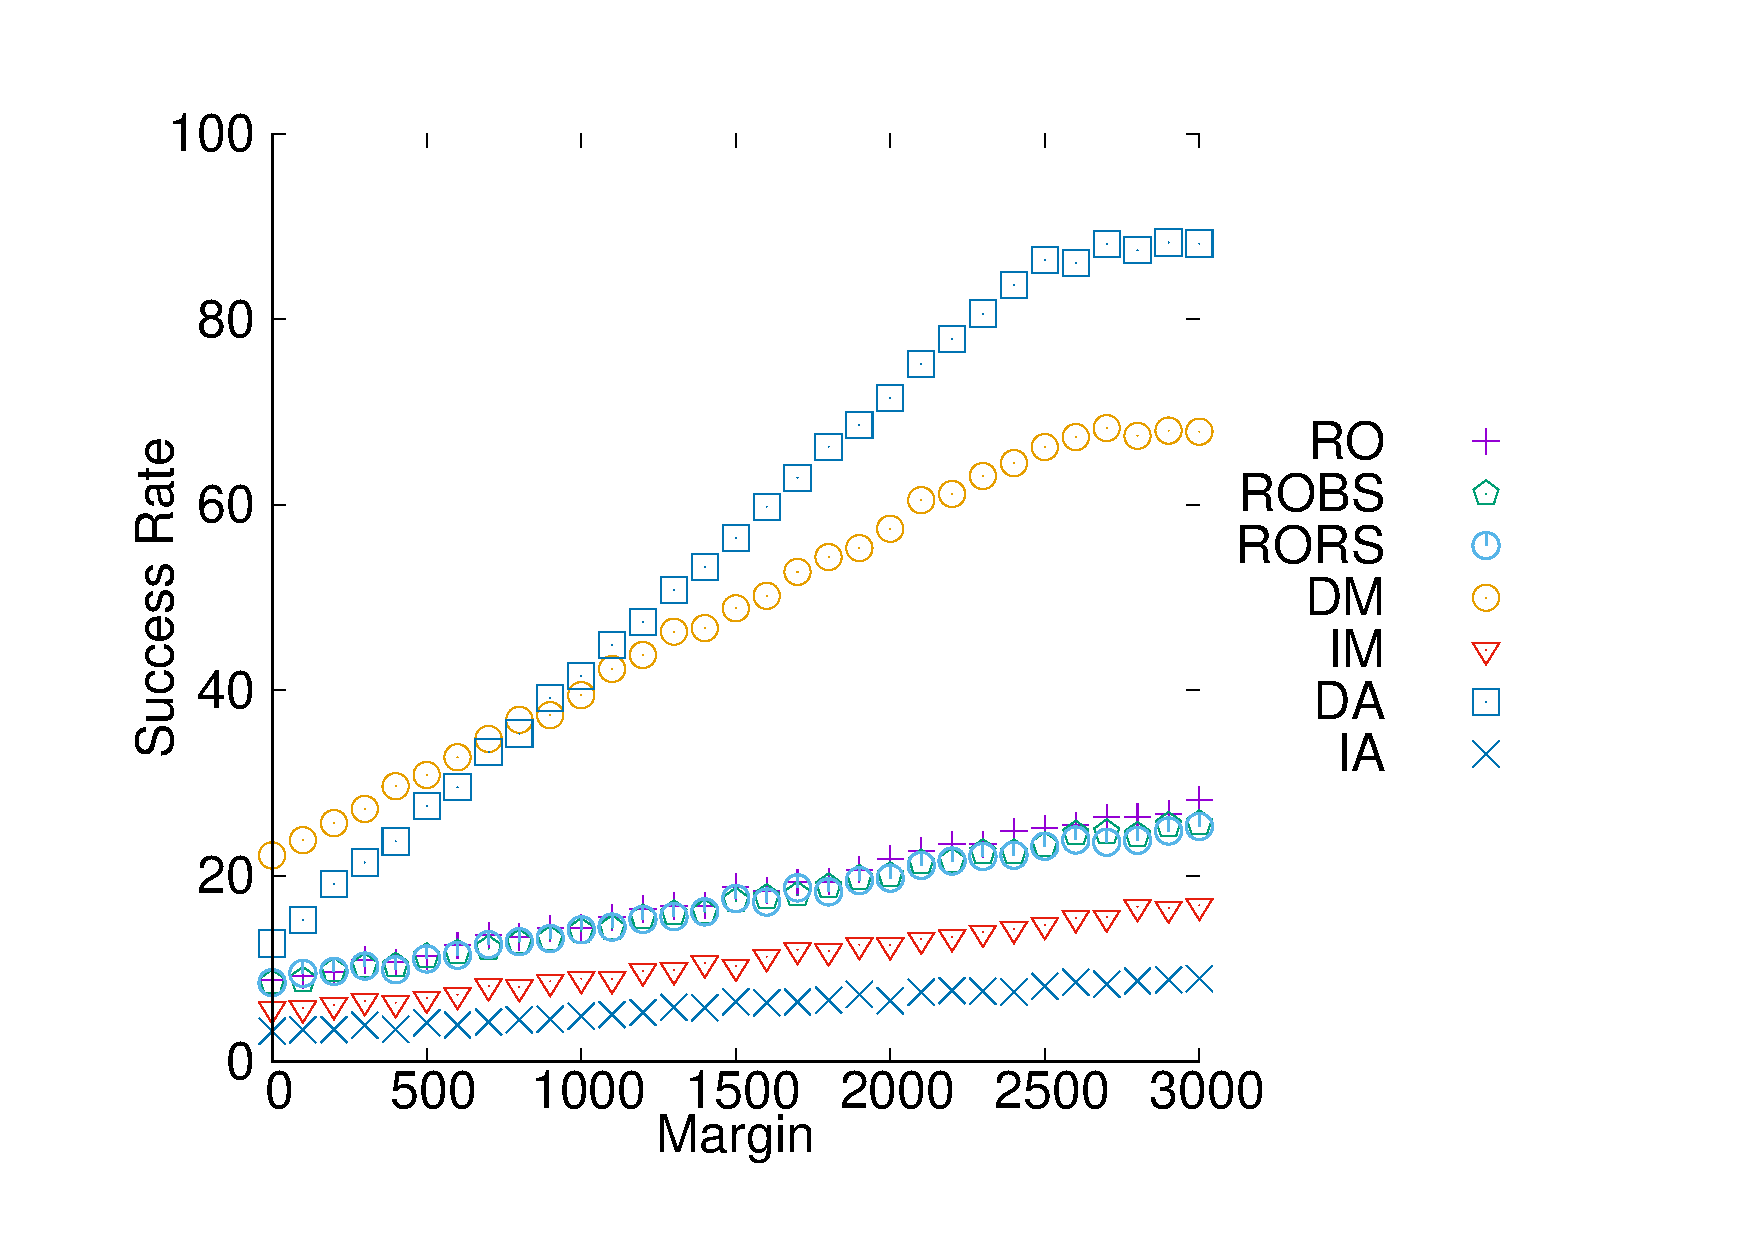
\includegraphics[width=0.45\textwidth]{Chapitre4/departs_gp_250001.pdf}
           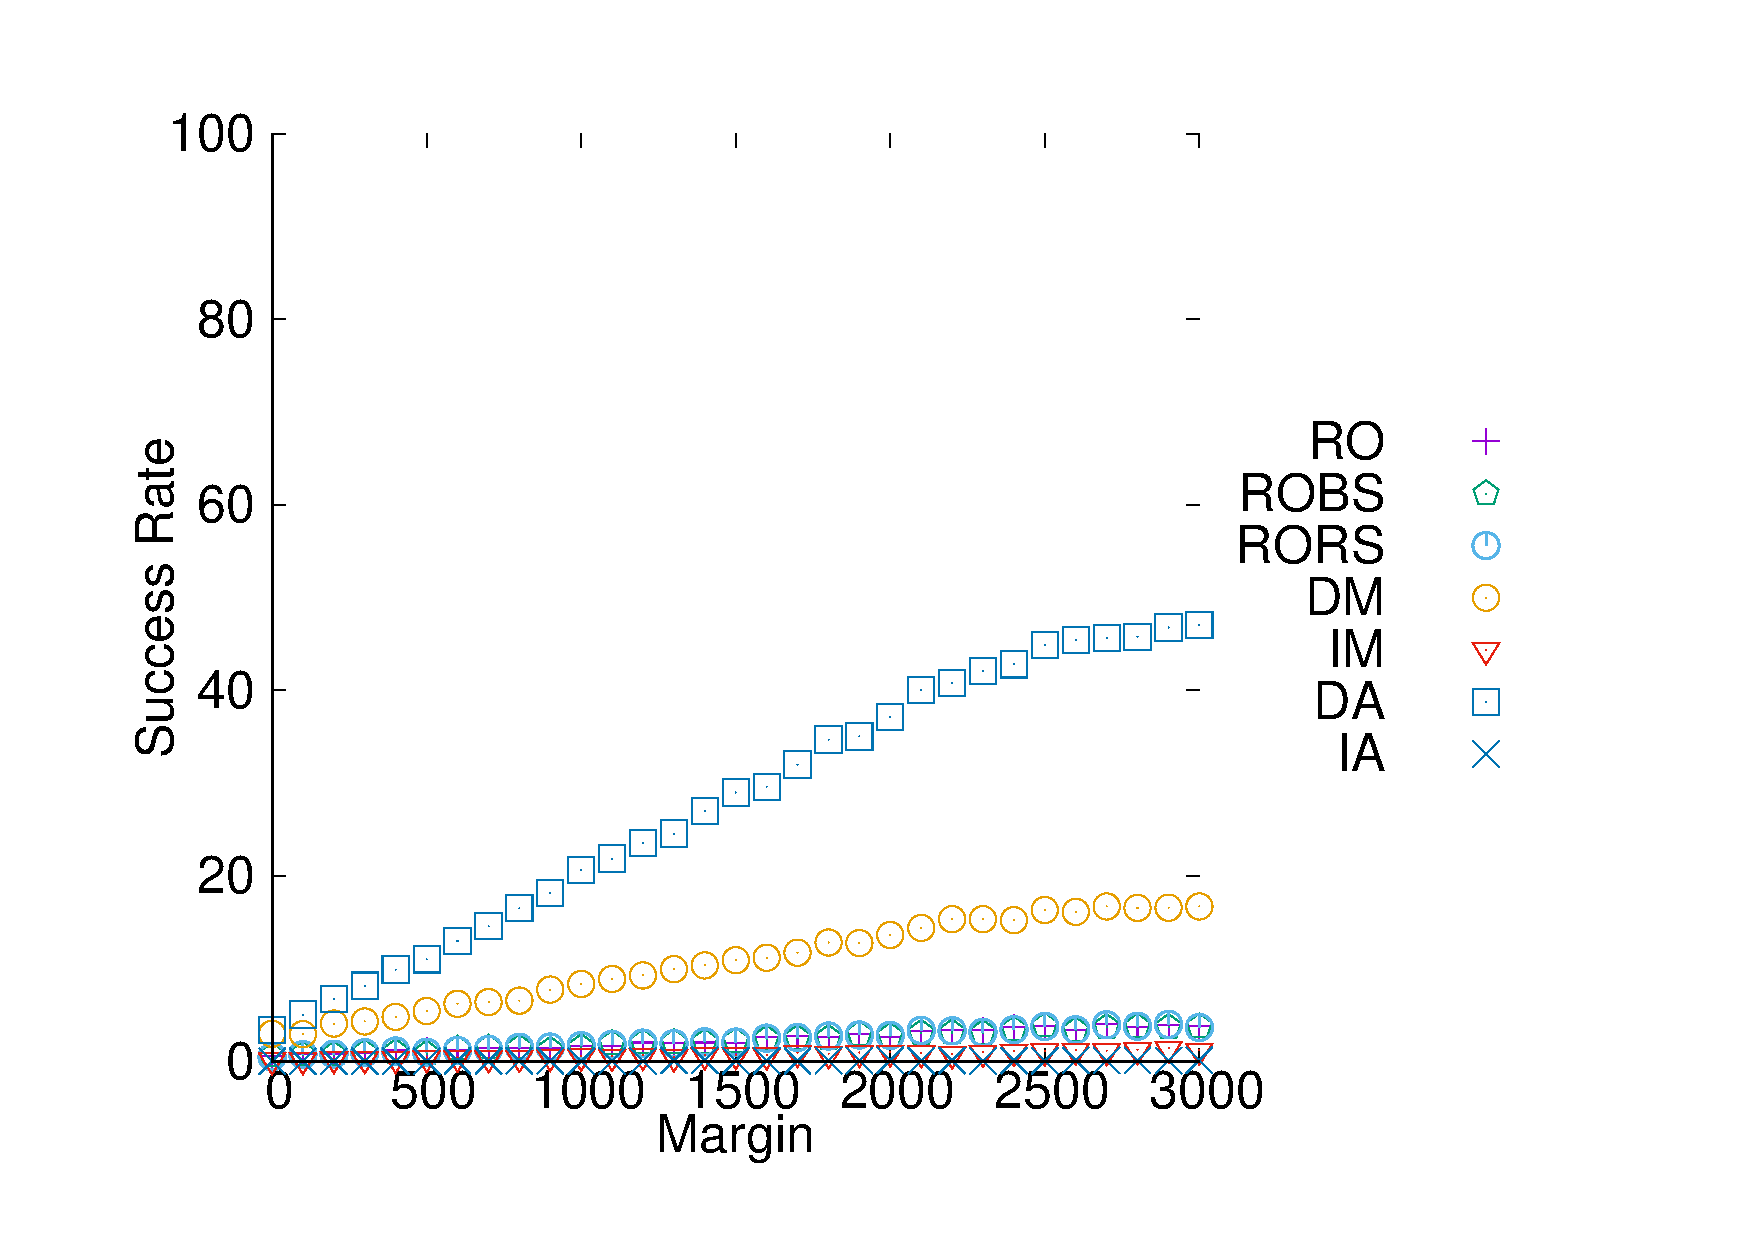
\includegraphics[width=0.45\textwidth]{Chapitre4/departs_gp_210001.pdf}
      \caption{Success rate of different sending orders, left $80\%$ load, right $95\%$ load.}
           \label{fig:success1random}
     \end{figure}

          
     According to our experiments, policy IA, that is sending the datagrams on increasing order on the lenght of the arcs $(c_1,c_2)$, does not work well. It corresponds to the policy of Proposition~\ref{prop:SL} which we already know to be bad for \pazl when the routes are long as in this experiment. Sending on decreasing order on the margin of the routes (DM) or on the length of the arcs $(c_1,c_2)$ (DA) work better and it seems that DA is better than DM, especially in a loaded network. 
     
     Remark that sending the datagrams using a random order does not perform well,
     but better than IM and IA, which shows that the latters are a poor choice for the first stage of our algorithm. The interest of using a random order is that we can draw many of them. In Figure~\ref{fig:success1000random} the same experiment is made for the three heuristics choosing an order at random, but we now draw $1,000$ different random orders and solve each induced \wta instance using \greedydeadline. The algorithm is considered to succeed as soon as a valid assignment is found for one order. Each random order drawn is used for RO, RORS and ROBS to make the comparison fairer.

\begin{figure}[h] 
  \centering
  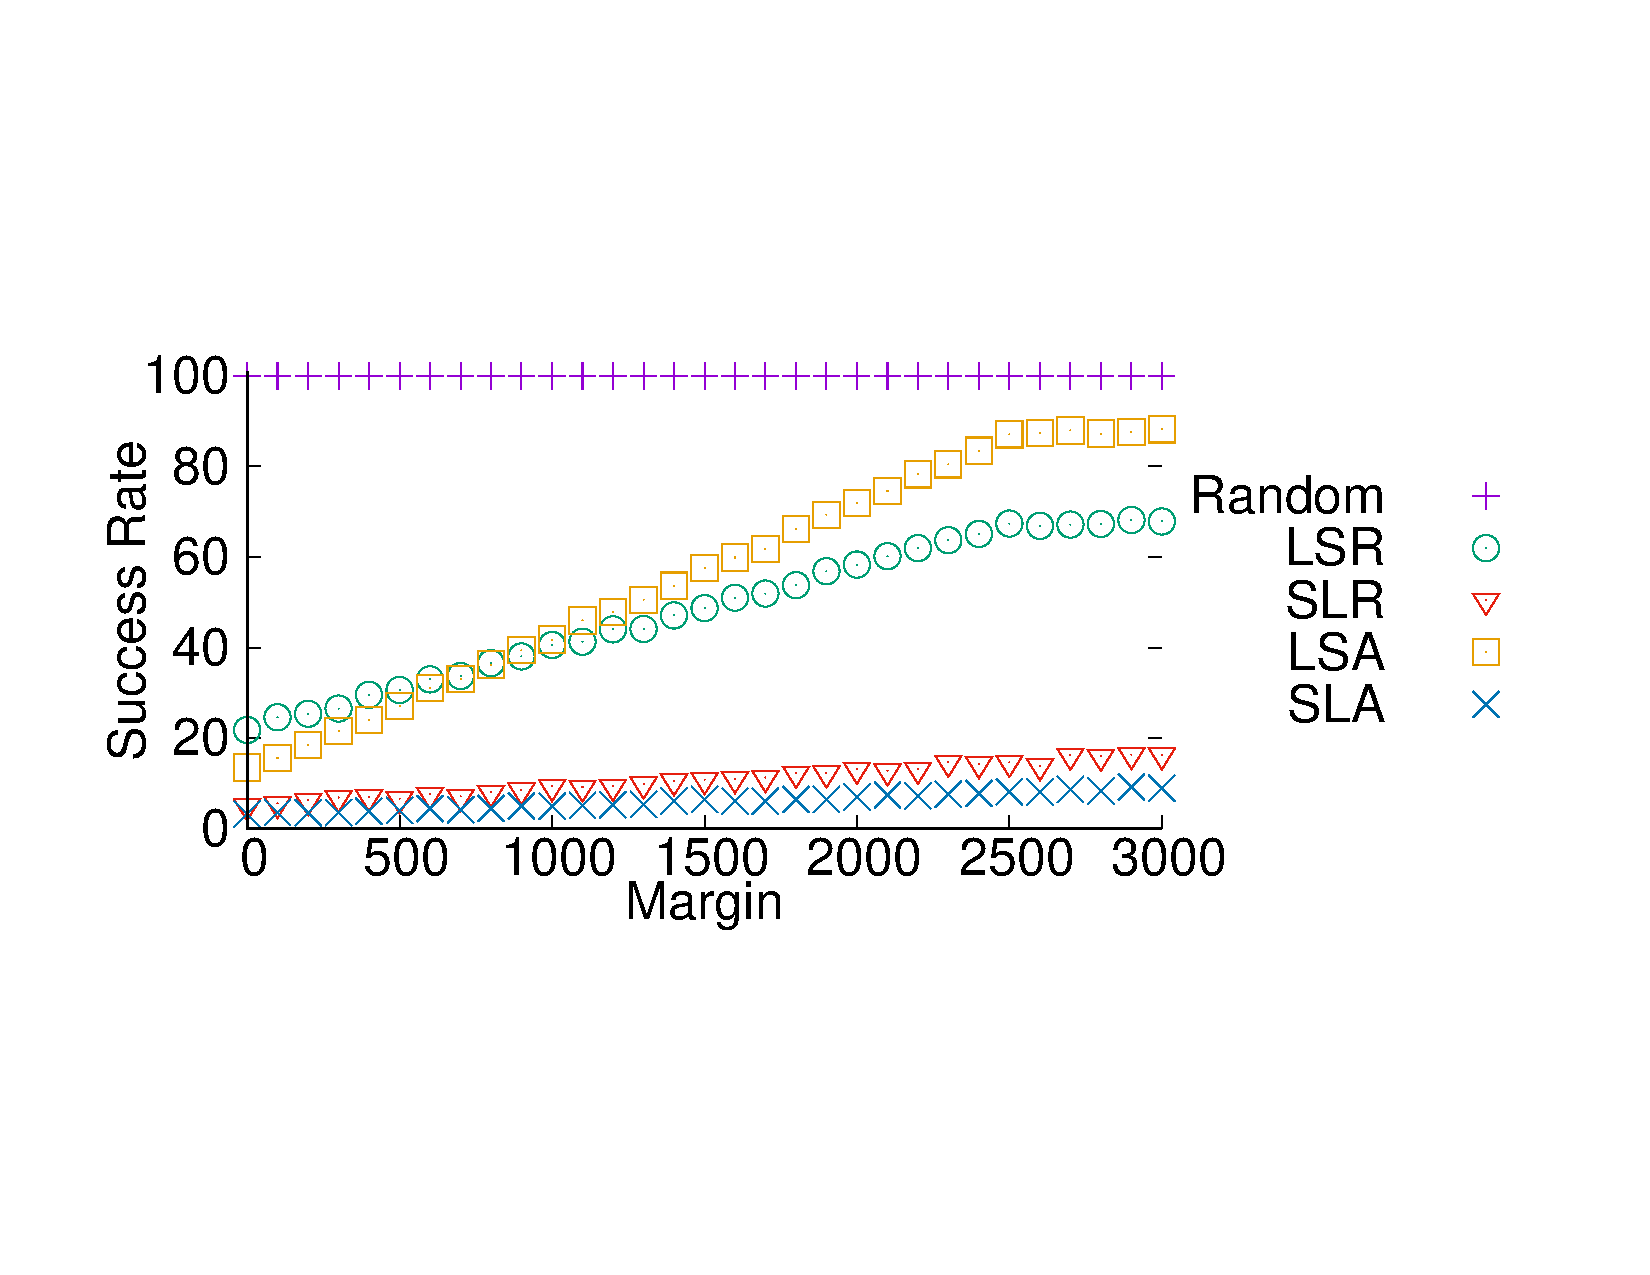
\includegraphics[width=0.45\textwidth]{Chapitre4/departs_gp_25000.pdf}
    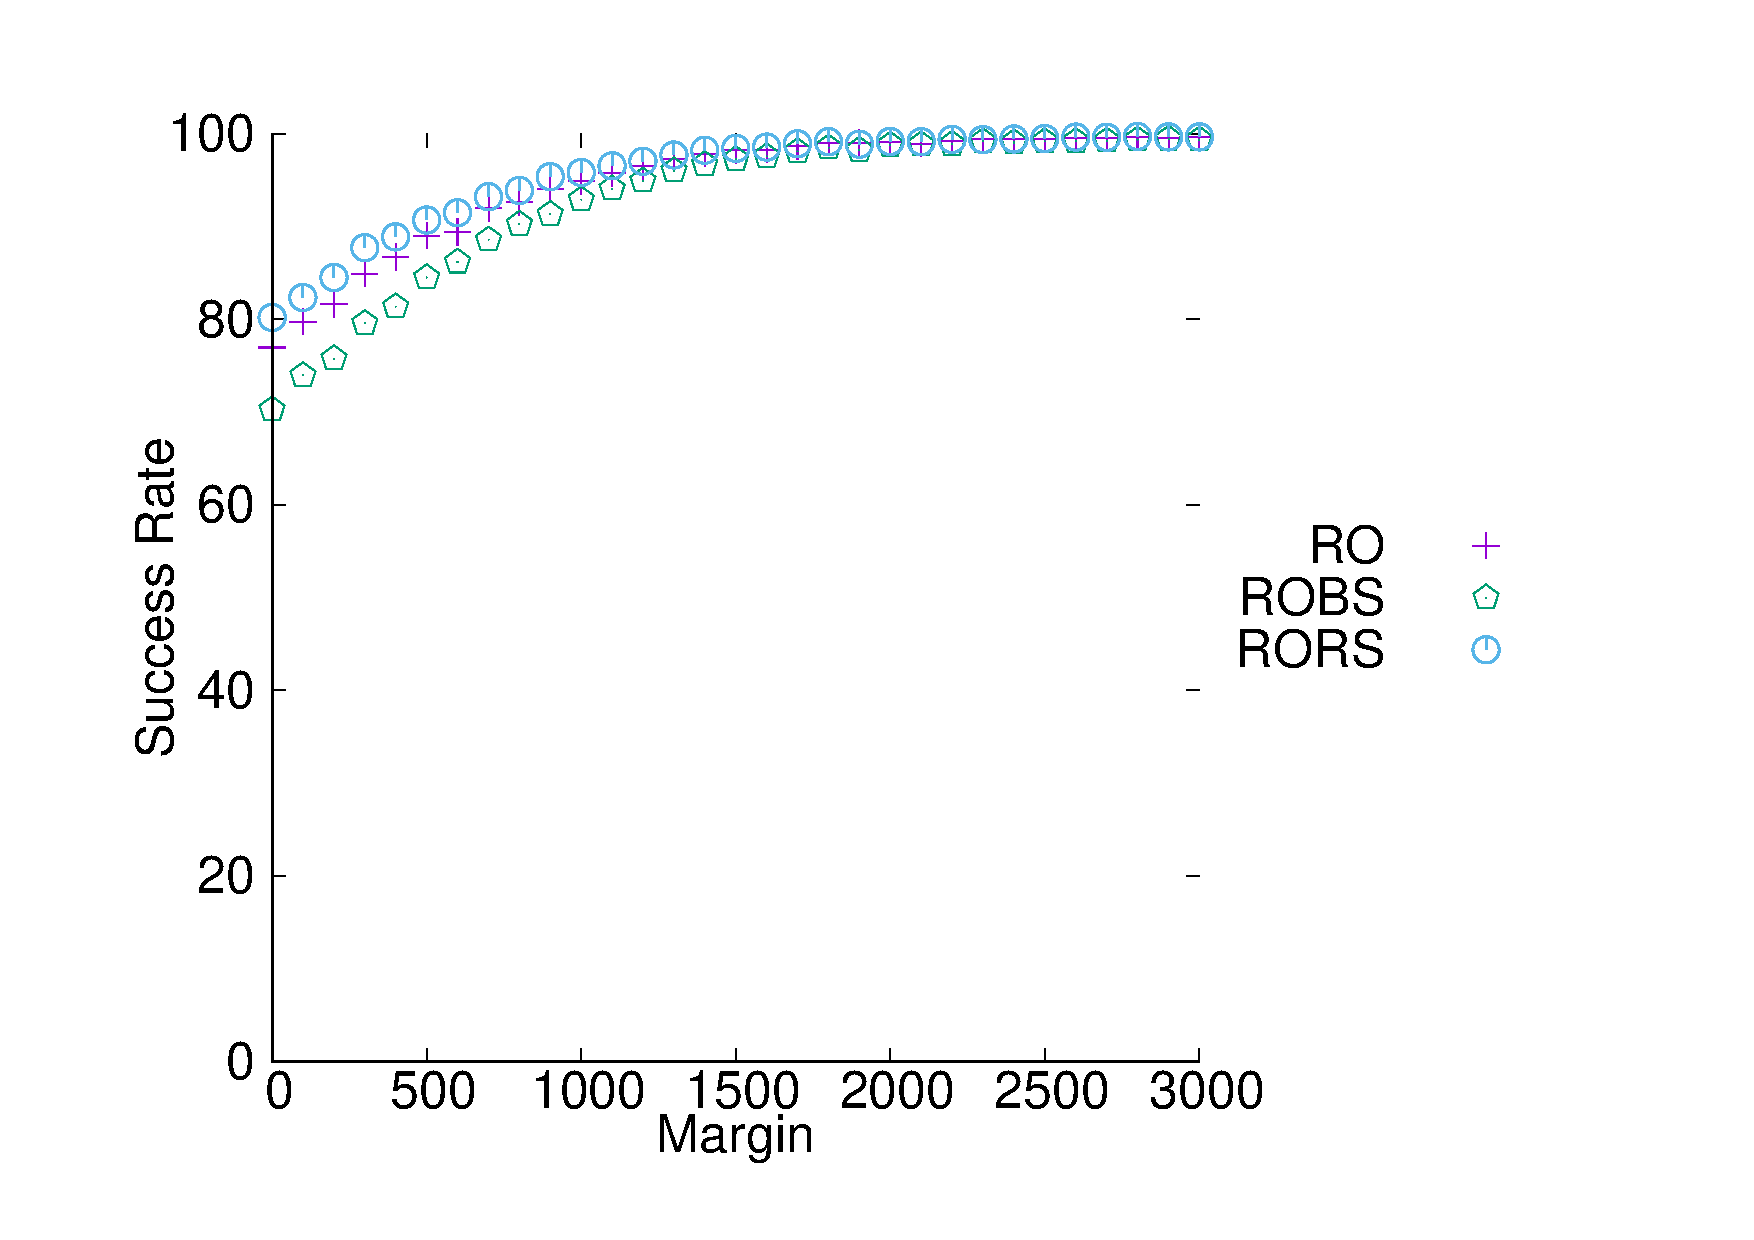
\includegraphics[width=0.45\textwidth]{Chapitre4/departs_gp_21000.pdf}
    
       \caption{Success rate of different sending orders with the random orders generated $1000$ times, left $80\%$ load, right $95\%$ load.}
      \label{fig:success1000random}
          \end{figure}

  First remark that our algorithms finds assignments with margin $0$ for instances with $95\%$ of load and long routes which was not possible when only looking for bufferless assignments (see Chapter~\ref{chap:PAZL}). It justifies the interest of studying \pall and not only \pazl.
  
     Using many random orders is much better than DA, the best policy using one specific order. 
     With a load of $95\%$, a solution is found with margin $0$ most of the time. The three random order policies have similar performances, but RORS has slightly better success rate than the two others ones, under high load and small margin. Hence, in the following experiments, we draw $1,000$ random orders using the policy RORS to set the offsets of the assignments.
     
      We now compare the performances of the four different algorithms used in the second stage to set the waiting times. Since \greedydeadline already finds assignments with margin $0$ on mild loads, it is more interesting to focus on the behavior of the algorithms with high load. In Figure~\ref{fig:success21000}, we represent the success rate of the four algorithms with regards to the margin, computed over $10,000$ random star routed networks generated with the same parameters as previously. 
     
    \begin{figure} [h] 
       \begin{center}
      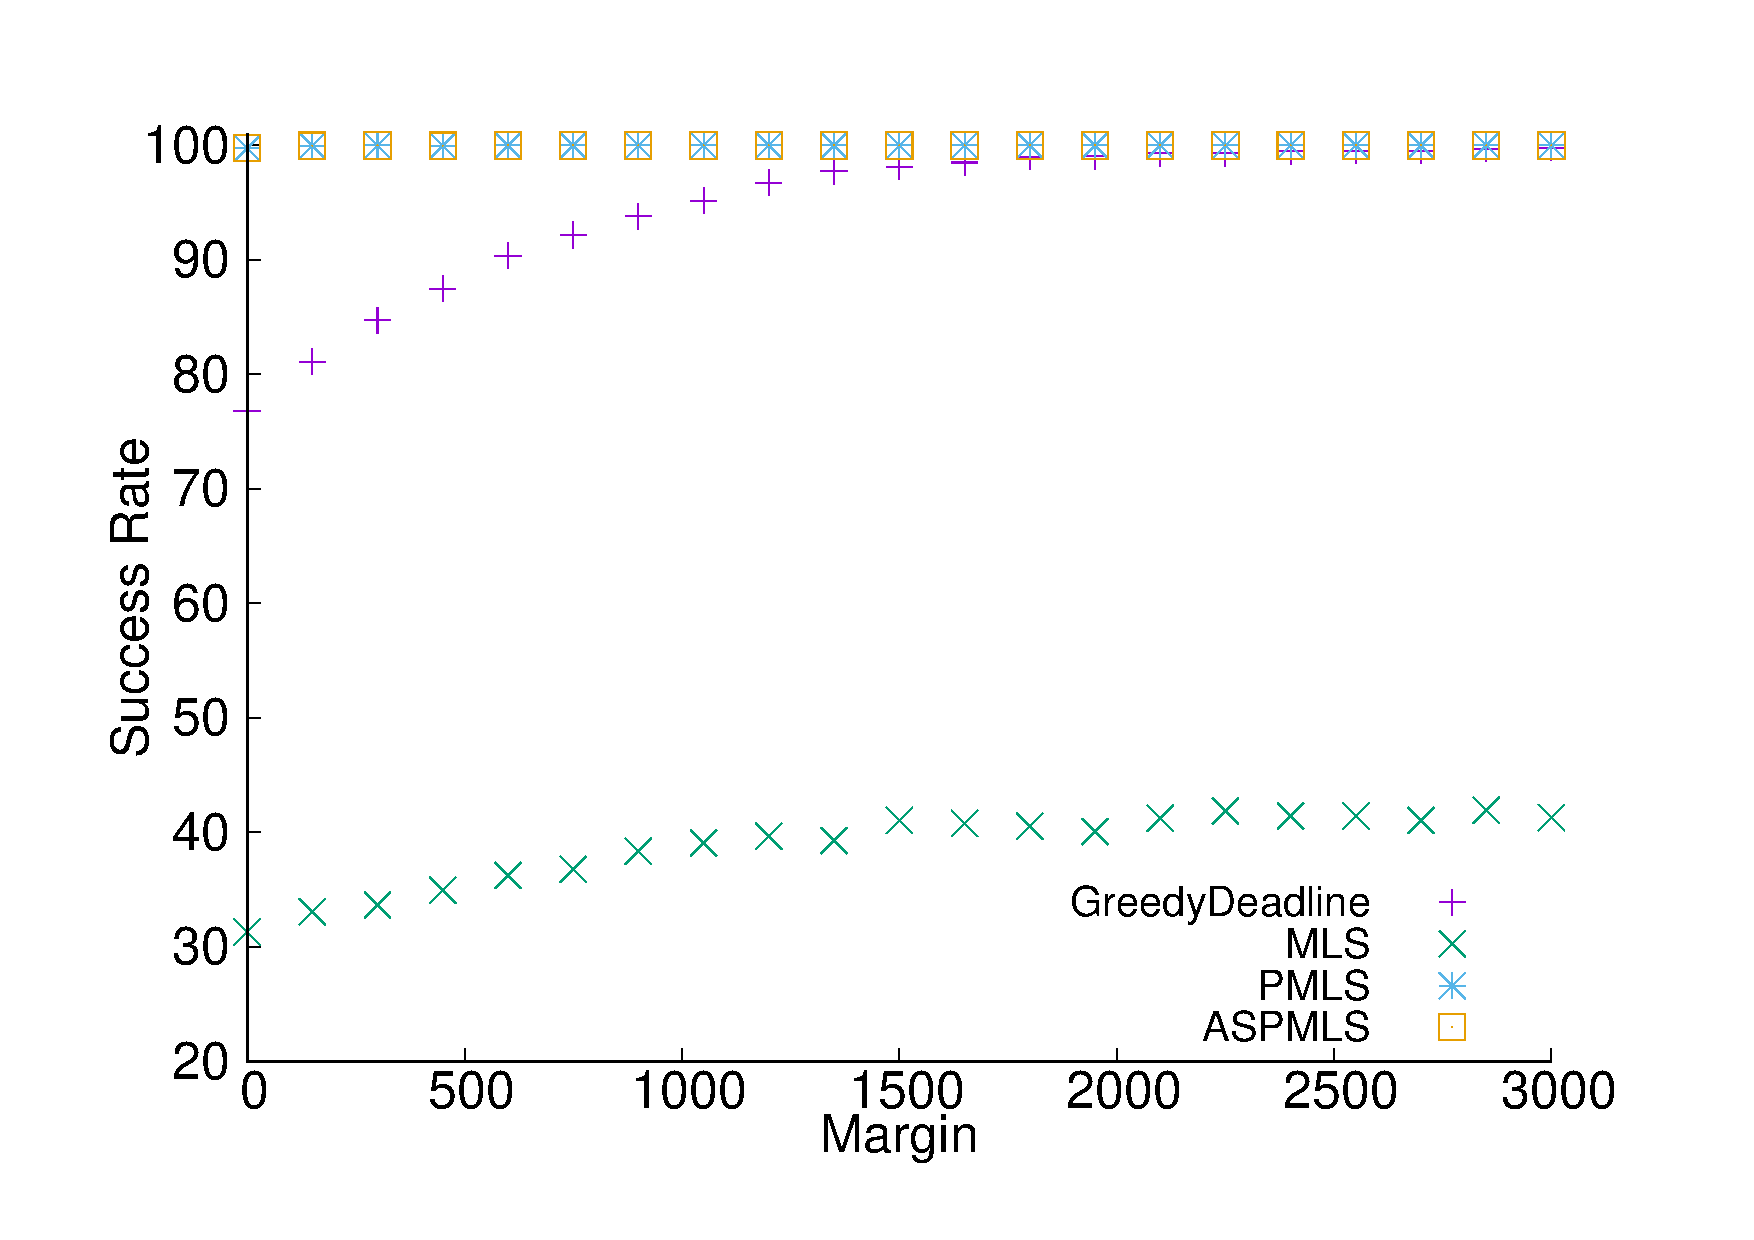
\includegraphics[width=0.5\textwidth]{Chapitre4/retour_21000.pdf}
      \end{center}
      \caption{Success rate of four algorithms solving \pall, $95\%$ load}
     \label{fig:success21000}
     \end{figure}
     
      The \MLS algorithm performs poorly, worst than \greedydeadline, \PMLS and \ASPMLS, which shows that \emph{taking into account the periodicity} is fundamental.
     Algorithm \greedydeadline is close to $100\%$ success rate for margins larger than $1,500$ while  \PMLS and \ASPMLS algorithms find a solution for more than $99\%$ of the random instances, even \emph{with a margin $0$}. In other words, for very high load and no margin, there are very few instances for which we do not find an assignment. With a margin of $300$, which corresponds to about $15\mu$s of additional delay with the chosen parameters, we always find a solution. 
     
     It turns out that the performances of \PMLS and \ASPMLS are almost identical. Even with a load of $100\%$ and a margin of $0$, we have to draw $100,000$ random instances before finding one which can be solved by \ASPMLS and not by \PMLS. Since \ASPMLS is of exponential complexity in $n$, it may not be relevant to use it within the parameters of this experiment. To verify that, we present the computing time of \PMLS and \ASPMLS for different instance sizes. To stress the algorithms, we set the margin to $0$ and the load to $95\%$. The table of Figure~\ref{fig:tps_fpt} shows the computation times of \PMLS and \ASPMLS, averaged on $1,000$ instances. 

     
          \begin{figure}[h] 
       \begin{center}
   \begin{tabularx}{0.8\textwidth}{|c|X|X|X|X|X|X|}
    \hline
    \# routes& $8$ & $12$ & $16$& $20$ & $24$\\
    \hline
    \ASPMLS (ms) & $1.88$ &$5.98$&$47.75$&$209.2$&$1815$\\
    \hline
     \PMLS (ms) & $0.07$ &$0.08$&$0.09$&$0.10$&$0.12$\\
    \hline
    Ratio & $27$ &$78$&$523$&$2122$&$14882$\\
    \hline
      \end{tabularx}
      \end{center}
   \caption{Computation time for \PMLS and \ASPMLS function of the number of routes}
        \label{fig:tps_fpt}
     \end{figure}
    

  The complexity of both these algorithm depends on the number of routes. As shown in Figure~\ref{fig:tps_fpt}, the time complexity of \PMLS seems linear on \emph{average}, while its theoretical worst case complexity is cubic. \ASPMLS scales exponentially with the number of routes as expected. Both algorithms are usable for instances of $20$ routes, but for $40$ routes or more \ASPMLS becomes too slow. Since \ASPMLS almost never finds a solution when \PMLS does not and is much slower, one should prefer to use \PMLS. 

    When evaluating the computing time of our method, we should take into account how many random orders are drawn. In previous experiments, we have drawn $1,000$ random orders which may be $1,000$ time slower than using a single fixed order. There is a trade-off between the number of random orders and the success rate. We investigate the success rate of our algorithms with regards to the number of random orders drawn, a load of $95\%$ and a margin $0$. The table of Figure~\ref{fig:randomdrawing} presents the success rate for different numbers of sending orders, averaged over $10,000$ instances, for \greedydeadline, \PMLS and \ASPMLS.


         \begin{figure}[h] 
       \begin{center}
   \begin{tabularx}{0.8\textwidth}{|c|X|X|X|X|X|X|}
    \hline
    \# orders& $1$ & $10$ & $100$& $1,000$& $10^{4}$&$10^{5}$\\
    \hline
    \greedydeadline & $0.55$ &$6.05$&$35.44$&$77.43$&$90.1$&$92.4$\\
    \hline
    \PMLS & $82.04$ &$98.84$&$99.71$&$99.80$&$99.83$&$99.83$\\
    \hline
    \ASPMLS & $91.33$&$99.17$&$99.72$&$99.80$ &$99.83$&$99.83$\\
    \hline
      \end{tabularx}
      \end{center}
   \caption{Success rates function of the number of random orders drawn}
        \label{fig:randomdrawing}
     \end{figure}

	First, observe that the better the algorithm to solve $\wta$ is, the less random orders it needs in stage one to achieve its best success rate. In particular, \ASPMLS has better results than \PMLS for less than $1,000$ random orders, but not beyond. This further justifies our choice to draw $1,000$ random orders, to obtain the best success rate within the smallest time.

	The number of different orders is $7!= 5,040$ since we have $8$ routes and the solutions are invariant up to a circular permutation of the order. Hence, for $8$ routes it is possible to test every possible order. However the computation time of this exhaustive method scales badly with $n$. The fact that \PMLS and \ASPMLS have already high success rates for $10$ random orders hints that even for a larger number of routes, drawing $1000$ random orders is sufficient to obtain good assignments.


     \paragraph{Harder Topologies}
     
    Previous experiments use instances with weights of arcs uniformly drawn in a large interval. However, it is quite natural to consider that most routes are of roughly the same length or can be arranged in two groups of similar lengths, when the fronthaul network involves one or two data-centers.
    
	  By Proposition~\ref{prop:asym}, there is an assignment with margin equal to the maximum difference
    between the sizes of the routes. Hence, if all routes have almost the same size, the needed margin is small. If the routes are drawn uniformly in a large interval, then the expected difference between the longest route and the second longest is large. This difference can be seen as a free waiting time for most routes, hence we expect to need little margin in this regime too. As a consequence, the harder instances should be for routes with length drawn in an interval of moderate size compared to the period.

  	Figures~\ref{fig:1grp} and~\ref{fig:2grp} show the probability of success of \PMLS  over $10,000$ instances as a function of the margin. In Figure~\ref{fig:1grp} the length of arcs are drawn in $[0,I]$, where $I$ goes from $0$ to $6400$. As expected the success rate decreases when the size of the interval increases, until $I = 1600$, and then increases again.  In the most difficult settings, only $78\%$ of the instances can be solved with margin $0$, and we need a margin of $1,900$ to ensure that \PMLS always finds a solution. Remark that \ASPMLS does not yields better results on these hard instances.

 	In Figure~\ref{fig:2grp}, we do the same experiment, except that the weights of arcs of half of the routes is drawn in $[I]$ and the length of the other half is drawn in $[P/2,P/2 + I[$. The situation is the same as for the previous experiment but with better success rates, hence the case of two data centers is simpler to deal with.
  
           \begin{minipage}{0.47\linewidth}

    
       \begin{center}
      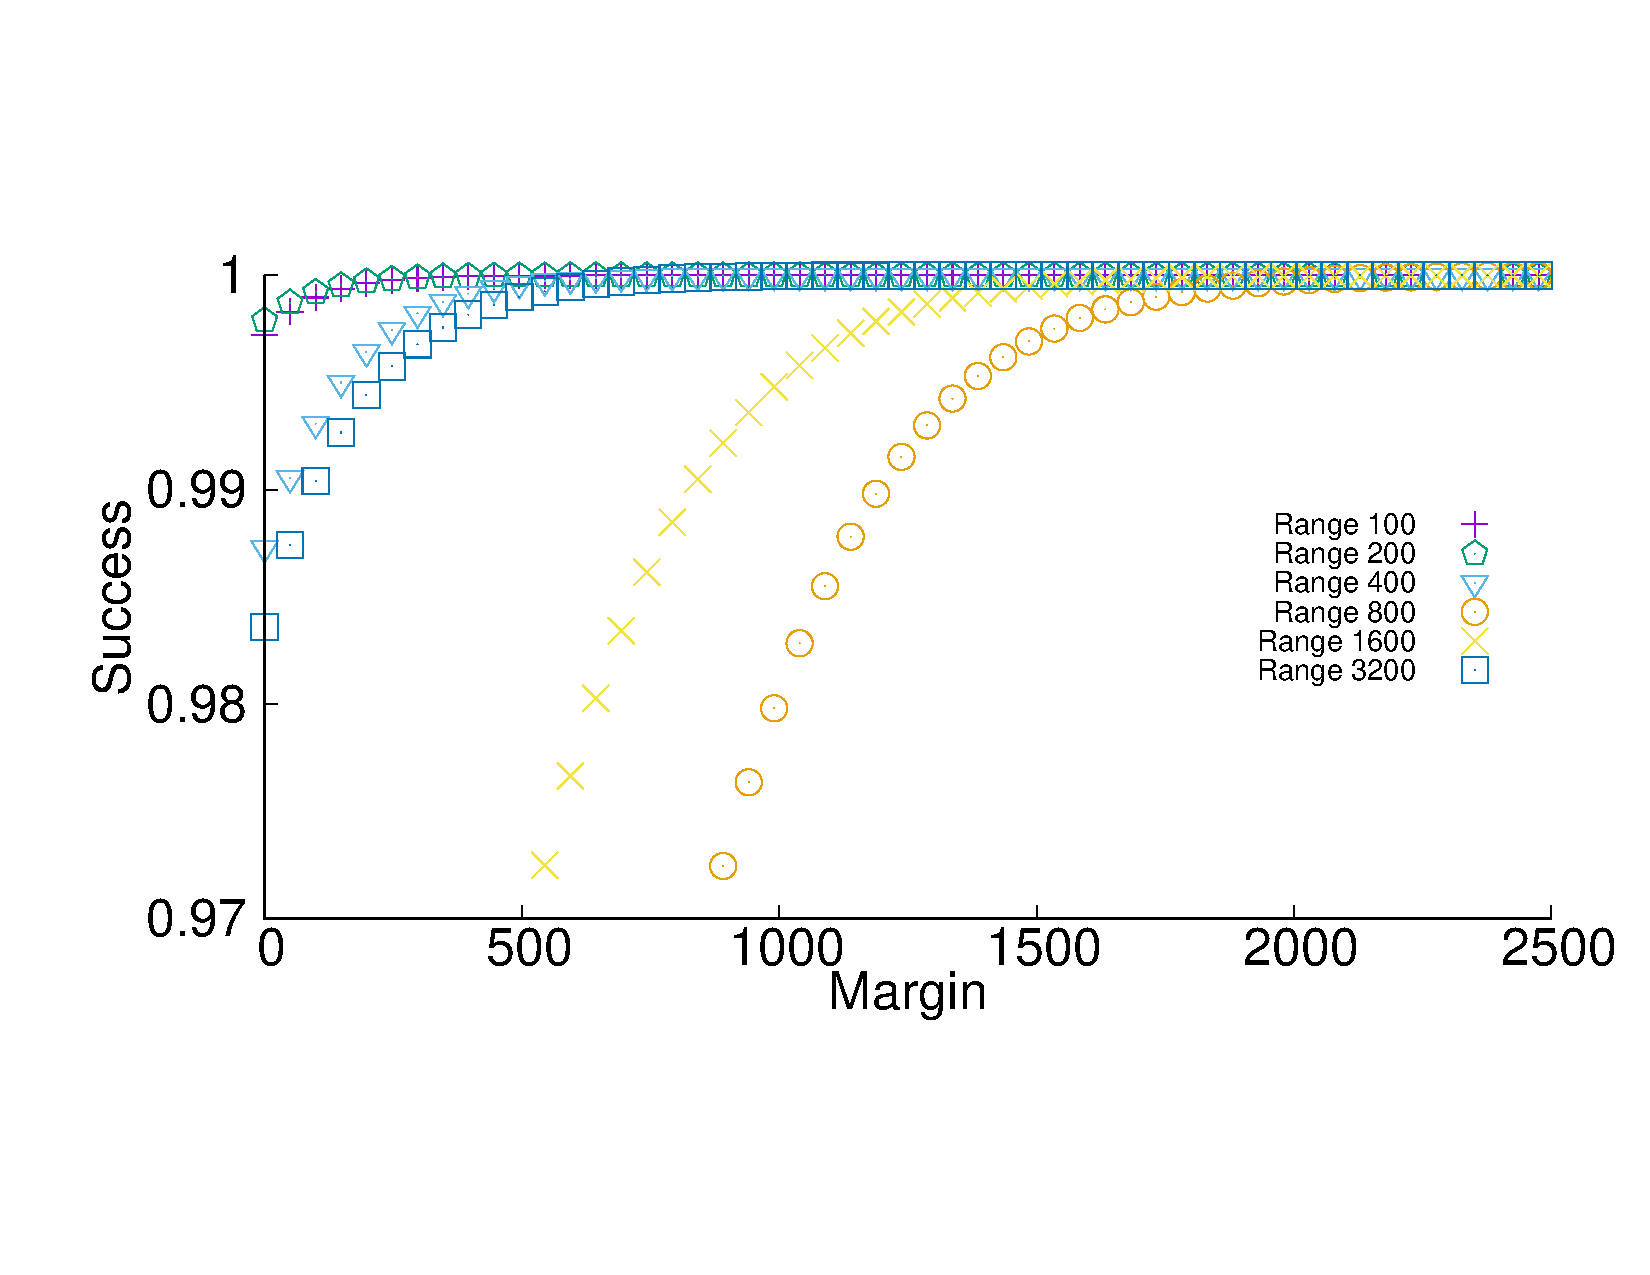
\includegraphics[width = \textwidth]{Chapitre4/departs_distrib1Grp.pdf}
     
      \captionof{figure}{Success rate of \PMLS, with length of arcs drawn in $[I]$}
      \label{fig:1grp}   
     
 \end{center}
   \end{minipage}\hfill
\begin{minipage}{0.47\linewidth}   
         
       \begin{center}
      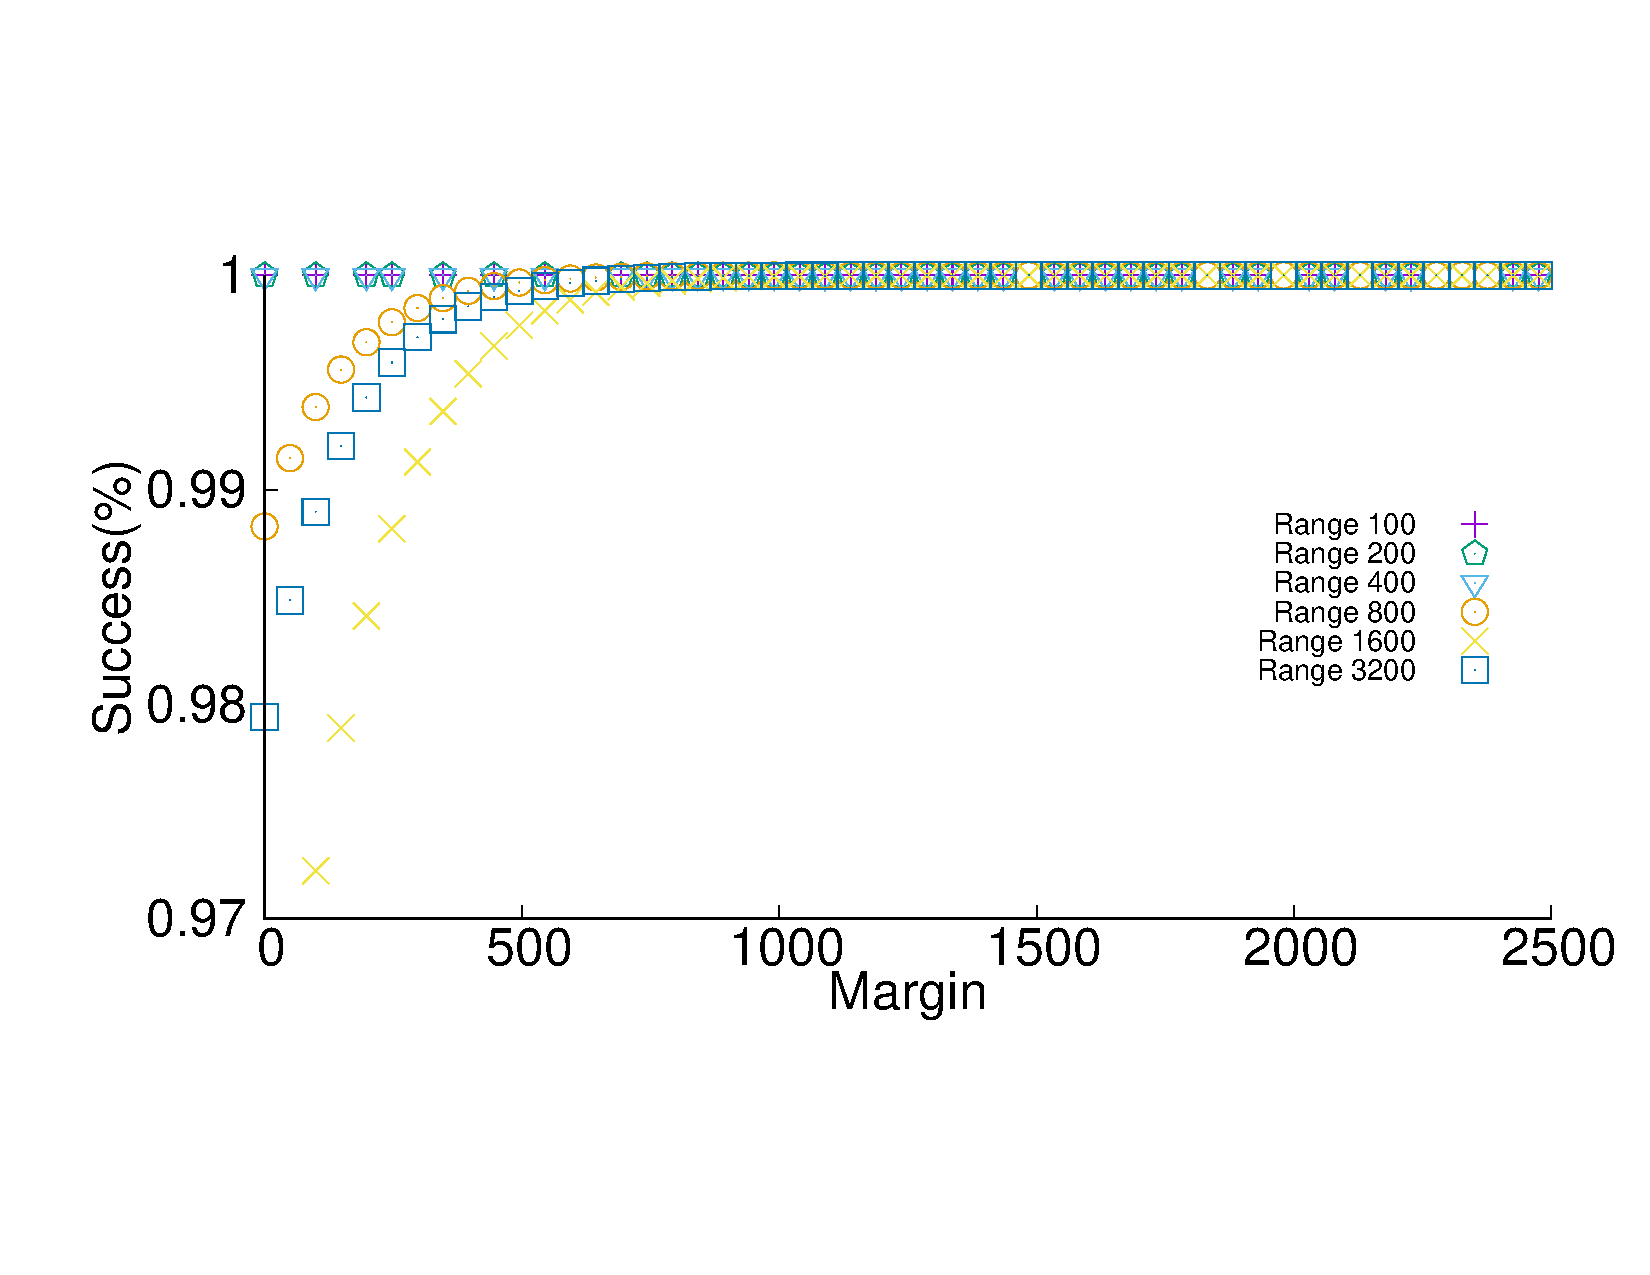
\includegraphics[width = \textwidth]{Chapitre4/departs_distrib2Grp.pdf}
   
    \captionof{figure}{Success rate of \PMLS, with length of arcs drawn in $[I]$ and $[P/2,P/2 + I[$}
      \label{fig:2grp}   
         \end{center}
      \end{minipage}\hfill
     

\section{Conclusion}

